\documentclass{article}
\usepackage{lmodern}
\usepackage[T1]{fontenc}
\usepackage[english,activeacute]{babel}
\usepackage{mathtools}
\usepackage{biblatex}
\usepackage{csquotes}
\usepackage{graphicx}

\title{User Behavior Analysis in Campus Area Networks through Kohonen Self Organizing Feature Maps}

\author{Nelson Victor Cruz Hern\'andez }

\date{May 2017}

\begin{document}

\maketitle

\section{Introduction}

\subsection{Antecedentes}

\maketitle

\section{Introduction}

\subsection{Antecedentes}

\subsection{Justification}

\subsection{Problem}

\subsection{Hypothesis}

\subsection{Objectives}

\subsubsection{General}

\subsubsection{Particular}

\section{State of the Art}

\subsection{Machine Learning Algorithms y Seguridad Inform�tica}

\subsection{Profiling / User classification}

\section{Marco Te�rico}

Local Area Network

Campus Area Network

Proxy

Stop condition

Epoch

\subsection{Redes de Computadoras}

\subsubsection{Network topology}

\subsubsection{OSI Model / TCPIP}

\subsubsection{Network Security}

\subsubsection{Intrusion Detection Systems}

\subsection{Machine Learning Algorithms}

\section{Desarrollo Metodol�gico}

\subsection{Experiment context}
Experiment was carried out on a Campus Area Network (CAN) that has a 16-bit network and a Windows domain controller, using a HTTP proxy. Among campus applications web and remote apps are included. Email service is provided by Microsoft Exchange Server which is hosted outside the campus network.
The target users were full-time professors who had a computer with a static IP address and a wireless access with a dynamic IP address.
Five full-time professors (hereafter denoted as users). were selected for the experiment. For each one, real traffic was captured during a week, and then processed.

\subsection{Explanation}
Self Organized Maps (SOM) algorithm works as an unsupervised learning clustering approach, where training is entirely data-driven and no target results for the input data vectors are provided. It also provides a topology to preserve mapping from high dimensional space to nodes (neurons) that form a two-dimensional lattice that represents high dimensional space onto a plane in which map units are grouped by it's features values similarity. Each node has a specific topological position and contains a vector weights (features) of the same dimension as the input vector [8].

Learning algorithm of Conventional SOM
1) Initialize the map using random vectors.

2) Searching for the winner unit
Select an input vector x randomly from learning set.
Search for the unit ???? which is associated to the closest vector ???? to x which minimize the quantization error |x ? m|.

3) Updating the winner unit and its neighboring units.
For the winner units ???? and its neighbor U ? w, update the vectors associated to the units using the following equation.
????=????+?????? �?� ???????
where ???? ?? is neighborhood function which is the decreasing function of distance d between ???? and ?????
and ? is the learning rate.

4) Repeat Step 2, Step 3 with decreasing neighborhood function ???? ?? and learning rate ? until the quantization error converges enough or during the pre-defined iterations

\subsection{Experiment execution}
The experiment has the goal of verifying if the behavior of an user in the network can be addressed as a pattern, and use it to determine if the activity in the network belongs to it, or not. Experiment is divided in four parts: data collecting, user activity processing into data chunks for data set creation, lattice training through SOM algorithm and obtained pattern evaluation. Fig. 1 shows the complete process.

\begin{center}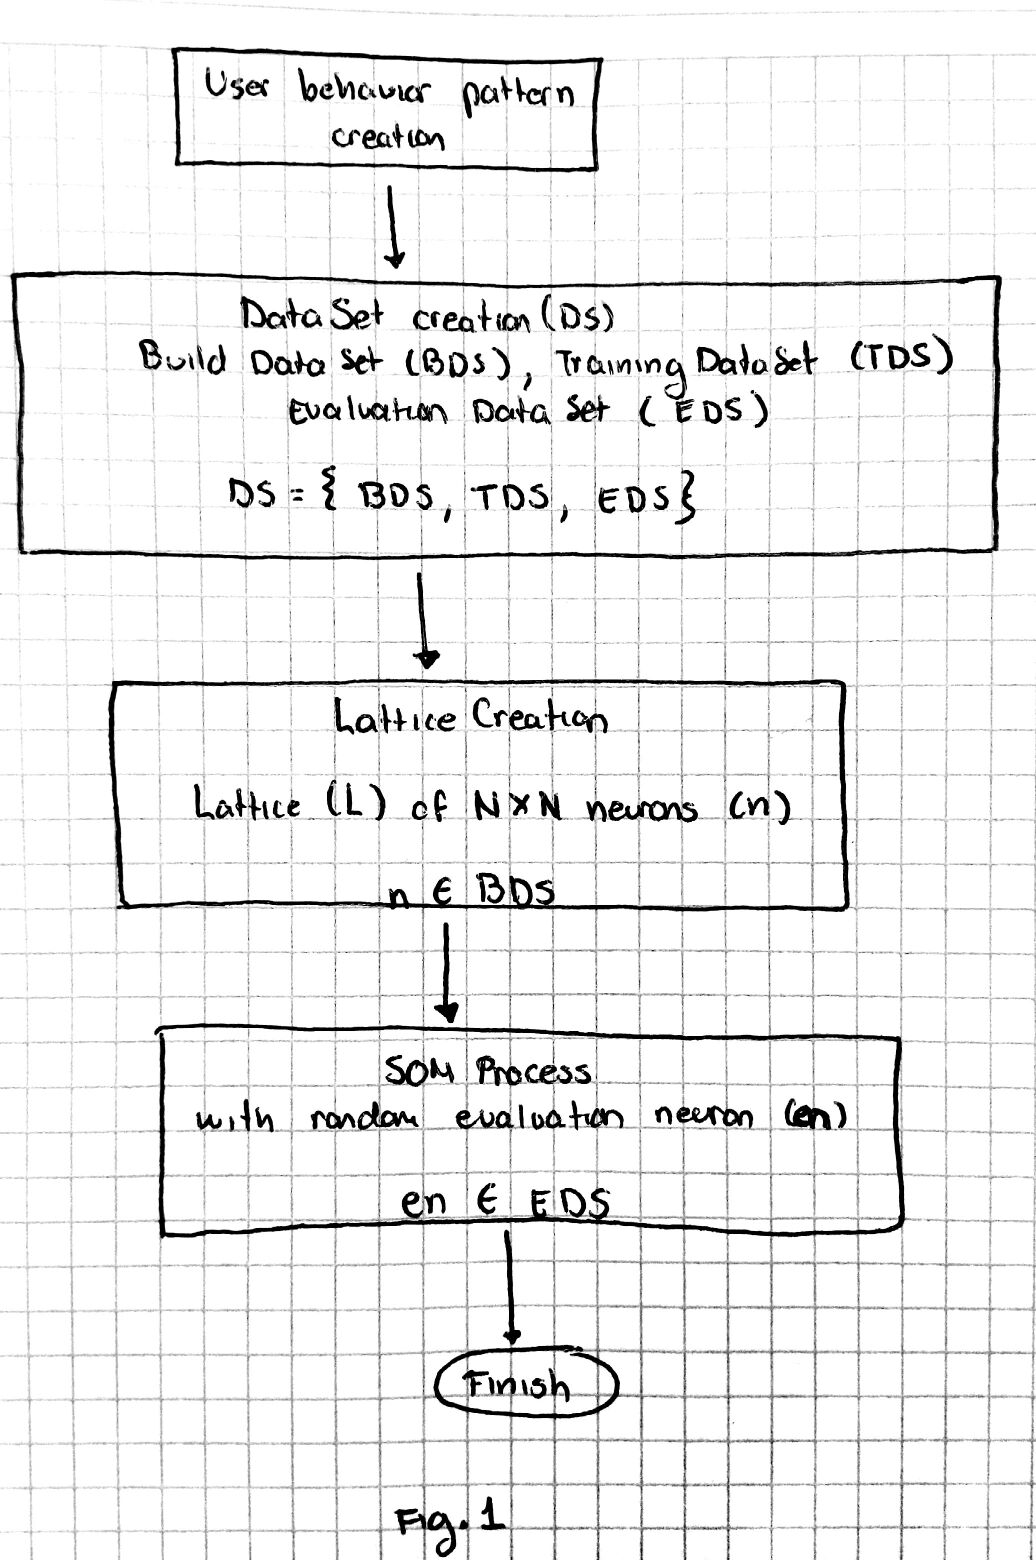
\includegraphics[scale=0.2]{fig-one} \end{center}

\subsubsection{Data collecting}
During a labor week, the normal behavior was captured from each user's computer. Before starting to capture, we checked that no computers had any malicious software installed. During this period only the owner user had access to each computer. The average size of of traffic captured was 3 gigabytes per user, involving more than four million packets, for each packet the following data is collected: way, origin IP, destination IP, used protocol, local used port, remote used port, total transmitted bytes and timestamp.

\subsubsection{User activity processing into data chunks for dataset creation}
Using packet as the unit for data evaluation is not an option due the great volume, and time consuming for processing \textbf{citation}, instead data is divided equally in three different types of datasets, one for building, other for training and the last for evaluation and then processed into data chunks. Fig 1.1 shows dataset creation.

\begin{center}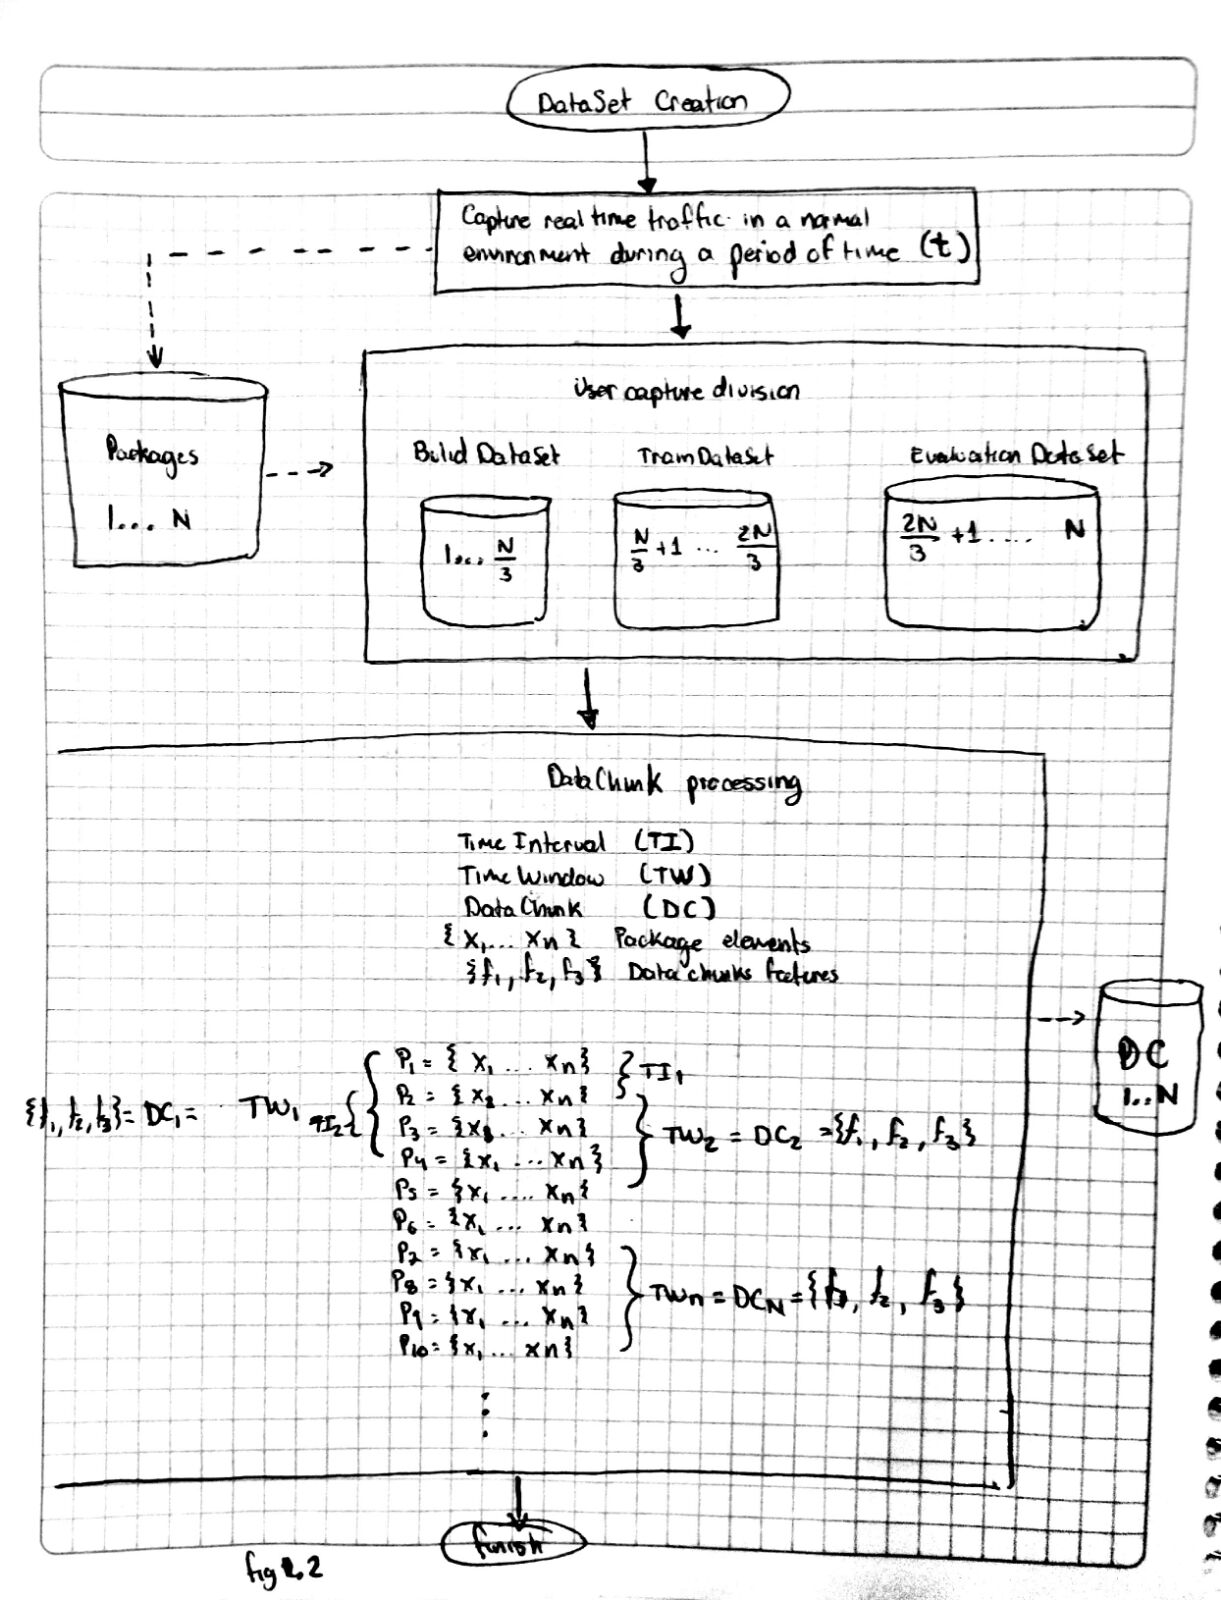
\includegraphics[scale=0.2]{fig-one-one} \end{center}

Each data set is created by 1...N data chunks. A data chunk has a set of continuous captured packages P1... P(N) which represents a fixed time window \textbf{\textit{tw}} of five minutes measured by the packet timestamp, in which three metrics are obtained: a) TCP/UDP metric, represents the ratio between total bytes sent through both protocols and total bytes sent in the chunk b) bytes to Internal IP metric, represents the ratio between total bytes sent to CAN proxy ip and total bytes sent in the chunk and c) web traffic metric, represents the ratio between data sent through web ports, and and total bytes sent in the chunk. This metrics will be the features which SOM algorithm will arrange the clusters. After \textbf{\textit{tw}} is processed, a time interval \textbf{\textit{ti}} of 10 seconds is given to start the data chunk process creation until no more packages are available. Each dataset is conformed by XXX data chunks.

\subsubsection{Lattice training through SOM algorithm}
This phase creates a user network pattern that represents its behavior in the network. Many pattern instances could be created from the user build dataset, as elements for creating it are randomly selected. Each neuron of the lattice is represented by an element of the Build Data Set, in which features are the three mentioned metrics in section 5.3.2. The lattice is has an arrange of 100 x 100 neurons, and a stop condition if 10 epochs. 

\subsubsection{Obtained pattern evaluation}
Comparison between two different lattices of the same user
Comparison between different lattices of multiple users

\section{Results and Discussion}
Results presentation, how the results are interpreted, and what we can do with data

\section{Conclusions}

\subsection{Conclusions}

\subsection{Future work}

\section{Bibliography}
[8] Dozono, H., Itou, S., and Nakakuni, M. (2007). Comparison of the adaptive authentication systems for behavior biometrics using the variations of self organizing maps. International Journal of Computers and Communications, 1(4), 108-116.

\end{document}